\chapter{Korisnički zahtjevi}
\section{Opis stranica}
\subsubsection{Početna stranica}
Pri pokretanju web aplikacije prikazuje se početna stranica koja pruža korisniku osnovne informacije o web aplikaciji te usmjerava korisnika na prijavu u sustav. U gornjem dijelu stranice nalazi se navigacijska traka putem koje korisnik pristupa različitim stranicama ovisno o svojim ovlastima. 
\subsubsection{Prijava}
Omogućuje korisniku unos korisničkih podataka i prijavu u aplikaciju pomoću adrese elektroničke pošte i lozinke. Korisnik se u sustav može samo prijaviti, registraciju novih korisnika obavlja administrator. Prijavljen korisnik neće moći pristupiti ovoj stranici.
\subsubsection{Info}
Pruža korisniku detaljnije informacije o autoškoli te približava svrhu same aplikacije. Stranica usmjerava korisnika na slanje upita putem kontaktnog obrasca ako ima dodatnih pitanja ili se želi prijaviti u autoškolu. Kontaktnim podacima može se pristupiti i u podnožju stranice.
\subsubsection{Kontakt}
Sadrži obrazac koji korisnik ispunjava pomoću imena, adrese elektroničke pošte i poruke. Ispunjen obrazac se šalje autoškoli klikom na gumb "Pošalji" koja se zatim javlja s odgovorima na potencijalna pitanja.
\subsubsection{Profil}
Prikazuje korisničke podatke unesene pri registraciji korisnika. Potrebni korisnički podaci za registraciju su ime, prezime, uloga, adresa elektroničke pošte, broj mobitela i datum rođenja. Osim obaveznih podataka, može se unijeti i napomena/bilješka za pojedinog korisnika koja se kasnije može uređivati i brisati.
\subsubsection{Kalendar}
Stranica namijenjena primarno instruktorima i polaznicima autoškole.Omogućuje prikaz, dodavanje, uređivanje i brisanje događaja u kalendar svakog korisnika. Na stranici se također nalaze korisničke upute za previđeno korištenje kalendara. Od kandidata se očekuje unos vremenske raspoloživosti prema kojoj instruktor unosi vrijeme obuke u raspored.
\subsubsection{Napredak}
Prikazuje napredak kandidata uz detaljan opis ishoda svakog sata. Realizirani ishod zabilježen je u posebnoj bilješci za svaki sat koju unosi instruktor putem forme na unos održanih sati. Klikom na pojedinu stavku iz trake za napredak prikazuje se skočni prozor sa svim detaljima za pojedini sat. Detalji koje korisnik može vidjeti su naslov održanog sata, datum, status, bilješka fotografija odvožene rute.
\subsubsection{Kandidati}
Stranica "Kandidati" pruža jednostavan pregled svih kandidata u autoškoli i omogućuje pristup podacima željenog kandidata. Podaci kojima instruktor i administrator mogu pristupiti su korisnički podaci sa stranice "Profil", kalendar i napredak željenog kandidata.
\subsubsection{Instruktori}
Omogućava  jednostavan pregled svih instruktora u autoškoli i omogućuje pristup podacima željenog instruktora. Podaci kojima administrator može pristupiti su korisnički podaci sa stranice "Profil"  i kalendar željenog instruktora.




\section{Vrste korisnika}
Postoje četiri kategorije korisnika sustava: neregistrirani korisnik te registrirani korisnici u koje ubrajamo  polaznike autoškole, instruktore i administratora.
\subsubsection{Anoniman korisnik}
Web aplikacija "Vožnja +" neregistriranom korisniku pruža pristup sljedećim stranicama: početna stranica, stranica za prijavu i informacije te stranici za slanje kontaktnog obrasca.  Korisnik može pronaći dodatne kontakt informacije i u podnožju stranice svake. Navedenim stranicama korisnik pristupa putem navigacijske trake.
\subsubsection{Kandidat}
Kao i anoniman korisnik, kandidat ima pristup početnoj stranici i stranici s dodatnim informacijama. Ako polaznik želi stupiti u kontakt s autoškolom, može to učiniti slanjem kontaktnog obrasca kojem pristupa preko stranice "Info" ili putem kontaktnih podataka u podnožju stranice. Na stranici "Profil" korisnik ima pregled svojih korisničkih podataka. Na toj stranici posebno se ističe mogućnost dodavanja i uređivanja bilješke ili napomene za svakog kandidata. Jedna od glavnih funkcionalnosti koje aplikacija pruža kandidatu je na stranici "Kalendar" gdje korisnik može dodavati, uređivati i brisati događaje što je posebno prikladno za označavanje vremenske raspoloživosti samog kandidata, a u istom kalendaru Korisnik može vidjeti termine koje mu je zakazao instruktor. Na stranici "Napredak" kandidat ima pristup traci za napredak putem koje se prati obuka kandidata. Klikom na odgovarajući element navigacijske trake, kandidatu je omogućen pregled bilješki za pojedini sat.
\subsubsection{Instruktor}
Poput kandidata, instruktor ima pristup početnoj stranici, kontaktnoj formi putem stranice "Info", stranici "Profil" s korisničkim podacima i stranici s vlastitim kalendarom. Dodatna mogućnost koju aplikacija pruža instruktoru je pregled svih kandidata, njihovim stranicama za napredak i kalendarima. Na stranici "Kandidati" instruktor odabire polaznika čijim podacima želi pristupiti. Najprije mu se prikazuje stranica s napretkom koju može uređivati tako da dodaje i uređuje bilješke za pojedini sat i samog kandidata, a klikom na gumb "Pogledaj kalendar" korisnika se preusmjerava na kalendar kandidata kojem on potom može upisivati, uređivati i brisati termine. Kalendari instruktora i kandidata su sinkronizirani što znači da će događaj koji instruktor upiše u kalendar polaznika biti vidljiv i u samom kalendaru instruktora.
\subsubsection{Administrator}
Administrator ima najveće ovlasti. Njegov primarni zadatak su registracija novih korisnika putem stranice "Registriraj" kojoj može pristupiti putem svoje navigacijske trake. Na stranicama "Instruktori" i "Kandidati" administratoru je omogućen jasan pregled svih korisnika sustava čijim podacima može pristupiti klikom na pojedinog korisnika. Administratoru je omogućen pregled korisničkih podataka sa stranica "Profil", događajima korisnika sa stranice "Kalendar" i napretku svakog kandidata putem stranice "Napredak". Osim privilegiranih funkcionalnosti, administrator ima pristup početnoj stranici, stranici i s dodatnim informacijama.
\newline
Svi registrirani korisnici se iz sustava odjavljuju odabirom opcije "Odjava" u navigacijskog traci.


\section{Obrasci uporabe}
Ključni scenariji interakcije između korisnika i aplikacije prikazat će se uz pomoć obrazaca uporabe. Svaki UC (engl. Use Case) pružit će jasno strukturirane korake koje korisnik slijedi te omogućit će nam razumijevanje odziva sustava na te korake. \\

\noindent \underbar{\textbf{UC1 - Pregled Info stranice}}
\begin{packed_item}
	
	\item \textbf{Glavni sudionik:} Neregistrirani/neprijavljeni korisnik i prijavljeni korisnik
	\item  \textbf{Cilj:} Pregled stranice s općim informacijama o web aplikaciji
	\item  \textbf{Sudionici:} -
	\item  \textbf{Preduvjet:} -
	\item  \textbf{Opis osnovnog tijeka:}
	
	\item[] \begin{packed_enum}
		
		\item Korisnik odabire opciju prikaza stranice Info
		\item Otvara se stranica i prikazuju informacije o web aplikaciji
		
	\end{packed_enum}						
\end{packed_item}

\noindent \underbar{\textbf{UC2 - Registracija}}
\begin{packed_item}
	
	\item \textbf{Glavni sudionik:} Administrator
	\item  \textbf{Cilj:} Stvaranje korisničkog računa za korištenje platforme
	\item  \textbf{Sudionici:} Baza podataka, Cloudinary
	\item  \textbf{Preduvjet:} Korisnik je prijavljen i ima ovlasti Administratora
	\item  \textbf{Opis osnovnog tijeka:}
	
	\item[] \begin{packed_enum}
		
		\item Korisnik odabire opciju registracije u navigacijskoj traci
		\item Korisnik unosi tražene podatke 
		\item Baza podataka se osvježava
		\item Korisnik dobiva  obavijest o uspješnoj registraciji te se osvježava forma za unos podataka
		
	\end{packed_enum}
	
	\item  \textbf{Opis mogućih odstupanja:}
	
	\item[] \begin{packed_item}
		
		\item[2.a] Unesena zauzeta e-mail adresa
		\item[] \begin{packed_enum}
			
			\item Obavijestiti korisnika o neispravnom unosu i omogućiti ponovni unos neprihvaćenih vrijednosti
			\item Korisnik unosi nove vrijednosti i uspješno završava registraciju ili odustaje od registracije 
			
		\end{packed_enum}
	\end{packed_item}
	
\end{packed_item}

\noindent \underbar{\textbf{UC3 - Prijava}}
\begin{packed_item}
	
	\item \textbf{Glavni sudionik:} Neregistrirani/neprijavljeni korisnik
	\item  \textbf{Cilj:} Dobiti pristup odgovarajućem korisničkom sučelju ovisno o ulozi 
	\item  \textbf{Sudionici:} Baza podataka
	\item  \textbf{Preduvjet:} Registracija od strane administratora, kontaktiranje autoškole
	\item  \textbf{Opis osnovnog tijeka:}
	
	\item[] \begin{packed_enum}
		
		\item Korisnik odabire opciju prijave u sustav
		\item Korisnik unosi tražene podatke (adresa elektroničke pošte i lozinka)
		\item Provjera ispravnosti unesenih podataka 
		\item Korisnik dobiva obavijest o uspješnoj prijavi i preusmjerava se na početnu stranicu za prijavljene korisnike 
		
	\end{packed_enum}
	
	\item  \textbf{Opis mogućih odstupanja:}
	
	\item[] \begin{packed_item}
		
		\item[2.a] Unesena neispravna adresa elektroničke pošte i/ili lozinka  
		\item[] \begin{packed_enum}
			
			\item Obavijestiti korisnika o neuspješnoj registraciji i omogućiti ponovni unos korisničkog imena i/ili lozinke
			\item Korisnik unosi nove vrijednosti i uspješno se prijavljuje ili odustaje od prijave
			
		\end{packed_enum}
	\end{packed_item}
	
\end{packed_item}

\noindent \underbar{\textbf{UC4 - Odjava}}
\begin{packed_item}
	
	\item \textbf{Glavni sudionik:} Prijavljeni korisnik (Administrator, Instruktor, Kandidat)
	\item  \textbf{Cilj:} Odjava iz sustava 
	\item  \textbf{Sudionici:} -
	\item  \textbf{Preduvjet:} Korisnik je trenutno prijavljen u sustav
	\item  \textbf{Opis osnovnog tijeka:}
	
	\item[] \begin{packed_enum}
		
		\item Korisnik odabire opciju odjave
		\item Korisnik gubi pristup korisničkim funkcijama
		\item Korisnik se preusmjerava na početnu stranicu za neregistrirane/neprijavljene korisnike 
		
	\end{packed_enum}
\end{packed_item}


\noindent \underbar{\textbf{UC5 - Pregled osobnih podataka}}
\begin{packed_item}
	
	\item \textbf{Glavni sudionik:} Prijavljeni korisnik (Administrator, Instruktor, Kandidat)
	\item  \textbf{Cilj:} Pregledati osobne podatke
	\item  \textbf{Sudionici:} Baza podataka
	\item  \textbf{Preduvjet:} Korisnik je trenutno prijavljen u sustav
	\item  \textbf{Opis osnovnog tijeka:}
	
	\item[] \begin{packed_enum}
		
		\item Korisnik odabire opciju za pregled svog profila
		\item Prikazuju se osobni podaci vezani uz korisnički račun
		
	\end{packed_enum}
\end{packed_item}


\noindent \underbar{\textbf{UC6 - Uređivanje osobne bilješke}}
\begin{packed_item}
	
	\item \textbf{Glavni sudionik:} Prijavljeni korisnik (Administrator, Instruktor, Kandidat)
	\item  \textbf{Cilj:} Izmijeniti bilješku na osobnom profilu 
	\item  \textbf{Sudionici:} Baza podataka
	\item  \textbf{Preduvjet:} Korisnik je trenutno prijavljen u sustav i otvoren mu je pregled osobnih podataka (\textbf{UC5})
	\item  \textbf{Opis osnovnog tijeka:}
	
	\item[] \begin{packed_enum}
		
		\item Korisnik odabire polje za unos bilješle
		\item Korisnik unosi/uređuje željeni tekst 
		\item Korisnik sprema promjene
		\item Baza podataka se osvježava 
		
	\end{packed_enum}
	
\end{packed_item}

\noindent \underbar{\textbf{UC7 - Slanje upita}}
\begin{packed_item}
	
	\item \textbf{Glavni sudionik:} Neprijavljeni korisnik i prijavljeni korisnik (Administrator, Instruktor, Kandidat)
	\item  \textbf{Cilj:} Poslati upit putem kontaktne forme 
	\item  \textbf{Sudionici:} EmailJS servis
	\item  \textbf{Preduvjet:} Korisnik je u navigacijskoj traci odabrao pristup stranici "Kontakt"
 (\textbf{UC5})
	\item  \textbf{Opis osnovnog tijeka:}
	
	\item[] \begin{packed_enum}
		
		\item Korisnik unosi tražene podatke
		\item Korisnik potvrđuje svoj zahtjev  
		\item EmailJS servis šalje ispunjenu kontaktnu formu autoškoli
		
	\end{packed_enum}
	
\end{packed_item}

\noindent \underbar{\textbf{UC8 - Pregled svih instruktorskih računa}}
	\begin{packed_item}
		
		\item \textbf{Glavni sudionik:} Administrator
		\item  \textbf{Cilj:} Prikaz svih instruktorskih računa 
		\item  \textbf{Sudionici:} Baza podataka
		\item  \textbf{Preduvjet:} Korisnik je trenutno prijavljen u sustav i ima ovlasti Administratora
		\item  \textbf{Opis osnovnog tijeka:}
		
		\item[] \begin{packed_enum}
			
			\item Administrator odabire opciju pregleda instruktorskih računa
			\item Prikazuje se popis svih instruktorskih računa
			
		\end{packed_enum}
		
	\end{packed_item}

 \noindent \underbar{\textbf{UC9 - Pregled svih kandidatskih računa}}
	\begin{packed_item}
		
		\item \textbf{Glavni sudionik:} Administrator i Instruktor
		\item  \textbf{Cilj:} Prikaz svih kandidatskih računa 
		\item  \textbf{Sudionici:} Baza podataka
		\item  \textbf{Preduvjet:} Korisnik je trenutno prijavljen u sustav i ima ovlasti Administratora ili Instruktora
		\item  \textbf{Opis osnovnog tijeka:}
		
		\item[] \begin{packed_enum}
			
			\item Korisnik odabire opciju pregleda kandidatskih računa
			\item Prikazuje se popis svih kandidatskih računa
			
		\end{packed_enum}
		
	\end{packed_item}

 \noindent \underbar{\textbf{UC10 - Pregled vlastitog kalendara}}
	\begin{packed_item}
		
		\item \textbf{Glavni sudionik:} Kandidat i Instruktor
		\item  \textbf{Cilj:} Prikaz kalendara 
		\item  \textbf{Sudionici:} Baza podataka
		\item  \textbf{Preduvjet:} Korisnik je trenutno prijavljen u sustav i ima ovlasti Kandidata ili Instruktora
		\item  \textbf{Opis osnovnog tijeka:}
		
		\item[] \begin{packed_enum}
			
			\item Korisnik odabire opciju pregleda svog kalendara
			\item Prikazuje se kalendar
			
		\end{packed_enum}
		
	\end{packed_item}

  \noindent \underbar{\textbf{UC11 - Uređivanje vlastitog kalendara}}
	\begin{packed_item}
		
		\item \textbf{Glavni sudionik:} Kandidat i Instruktor
		\item  \textbf{Cilj:} Uređivanje kalendara 
		\item  \textbf{Sudionici:} Baza podataka
		\item  \textbf{Preduvjet:} Korisnik je trenutno prijavljen u sustav, ima ovlasti Kandidata ili Instruktora i otvorena mu je stranica sa vlastitim kalendarom
		\item  \textbf{Opis osnovnog tijeka:}
		
		\item[] \begin{packed_enum}
			
			\item[1.a] Korisnik odabire postojeći vremenski interval 
                \item[1.b] Korisnik odabire željeni vremenski interval 
			\item Korisnik unosi/uređuje željeni naslov
                \item Korisnik potvrđuje svoj izbor
			
		\end{packed_enum}
		
	\end{packed_item}


\noindent \underbar{\textbf{UC12 - Pregled vlastitog napretka }}
	\begin{packed_item}
		
		\item \textbf{Glavni sudionik:}  Kandidat
		\item  \textbf{Cilj:} Prikaz stranice sa napretkom kandidata 
		\item  \textbf{Sudionici:} Baza podataka
		\item  \textbf{Preduvjet:} Korisnik je trenutno prijavljen u sustav i ima ovlasti Kandidata
		\item  \textbf{Opis osnovnog tijeka:}
		
		\item[] \begin{packed_enum}
			
			\item Kandidat odabire opciju pregleda vlastitog napretka
		
                \item Prikazuje se stranica sa napretkom kandidata
			
		\end{packed_enum}
		
	\end{packed_item}

 \noindent \underbar{\textbf{UC13 - Pregled napretka kandidata}}
	\begin{packed_item}
		
		\item \textbf{Glavni sudionik:} Administrator i Instruktor
		\item  \textbf{Cilj:} Prikaz stranice sa napretkom kandidata 
		\item  \textbf{Sudionici:} Baza podataka
		\item  \textbf{Preduvjet:} Korisnik je trenutno prijavljen u sustav i ima ovlasti Administratora ili Instruktora
		\item  \textbf{Opis osnovnog tijeka:}
		
		\item[] \begin{packed_enum}
			
			\item Iz popisa svih kandidata korisnik odabire željenog kandidata
                \item Prikazuje se stranica sa napretkom kandidata
			
		\end{packed_enum}
		
	\end{packed_item}

 \noindent \underbar{\textbf{UC14 - Pregled instruktorovog kalendara}}
	\begin{packed_item}
		
		\item \textbf{Glavni sudionik:} Administrator 
		\item  \textbf{Cilj:} Prikaz kalendara željenog korisnika
		\item  \textbf{Sudionici:} Baza podataka
		\item  \textbf{Preduvjet:} Korisnik je trenutno prijavljen u sustav i ima ovlasti Administratora 
		\item  \textbf{Opis osnovnog tijeka:}
		
		\item[] \begin{packed_enum}
			
			\item Admin odabire željenog instruktora iz popisa svih instruktora
			
                \item Prikazuje se stranica sa kalendarom željenog  korisnika
			
		\end{packed_enum}
		
	\end{packed_item}

 \noindent \underbar{\textbf{UC15 - Pregled kandidatovog kalendara}}
	\begin{packed_item}
		
		\item \textbf{Glavni sudionik:} Administrator i Instruktor
		\item  \textbf{Cilj:} Prikaz kalendara željenog korisnika
		\item  \textbf{Sudionici:} Baza podataka
		\item  \textbf{Preduvjet:} Korisnik je trenutno prijavljen u sustav, ima ovlasti Administratora ili Instruktora i prikazana mu je stranica Napredak željenog kandidata
		\item  \textbf{Opis osnovnog tijeka:}
		
		\item[] \begin{packed_enum}
			
			
			\item Korisnik na stranici Napredak odabranog kandidata odabire opciju prikaza kalendara
                \item Prikazuje se stranica sa kalendarom željenog  korisnika
			
		\end{packed_enum}
		
	\end{packed_item}


 \noindent \underbar{\textbf{UC16 - Uređivanje korisničkog kalendara}}
	\begin{packed_item}
		
		\item \textbf{Glavni sudionik:} Administrator i Instruktor
		\item  \textbf{Cilj:} Uređivanje  korisničkog kalendara 
		\item  \textbf{Sudionici:} Baza podataka
		\item  \textbf{Preduvjet:} Korisnik je trenutno prijavljen u sustav, ima ovlasti Kandidata ili Instruktora i otvorena mu je stranica sa korisničkim kalendarom
		\item  \textbf{Opis osnovnog tijeka:}
		
		\item[] \begin{packed_enum}
			
			\item[1.a] Korisnik odabire postojeći vremenski interval 
                \item[1.b] Korisnik odabire željeni vremenski interval 
			\item Korisnik unosi/uređuje željeni naslov
                \item Korisnik potvrđuje svoj izbor
			
		\end{packed_enum}
		
	\end{packed_item}


  \noindent \underbar{\textbf{UC17 - Prikaz bilješke za održani sat}}
	\begin{packed_item}
		
		\item \textbf{Glavni sudionik:} Prijavljeni korisnik (Administrator, Instruktor, Kandidat)
		\item  \textbf{Cilj:} Prikaz bilješke za održani sat obuke
		\item  \textbf{Sudionici:} Baza podataka
		\item  \textbf{Preduvjet:} Korisnik je trenutno prijavljen u sustav, ima ovlasti nekog od prijavljenih korisnika i otvorena mu je stranica sa napretkom
		\item  \textbf{Opis osnovnog tijeka:}
		
		\item[] \begin{packed_enum}
			
			\item Korisnik odabire željeni sat u traci napretka 
                \item[2.a] Prikazuje se bilješka za održani sat
                \item[2.a] Prikazuju se prazan skočni prostor - nema bilješke za odabrani sat
			
		\end{packed_enum}
		
	\end{packed_item}

 \noindent \underbar{\textbf{UC18 - Unos bilješke za održani sat}}
	\begin{packed_item}
		
		\item \textbf{Glavni sudionik:} Administrator i Instruktor
		\item  \textbf{Cilj:} Unos bilješke za održani sat obuke
		\item  \textbf{Sudionici:} Baza podataka
		\item  \textbf{Preduvjet:} Korisnik je trenutno prijavljen u sustav, ima ovlasti Administratora i Instruktora otvorena mu je stranica sa napretkom
		\item  \textbf{Opis osnovnog tijeka:}
		
		\item[] \begin{packed_enum}
			
			\item Korisnik odabire opciju unosa bilješke za željeni sat 
                \item Korisnik unosi tražene podatke
                \item Korisnik potvrđuje svoj izbor 
                \item Ažurira se baza podataka 
                
			
		\end{packed_enum}
		
	\end{packed_item}

 \noindent Na slici 1.1 možemo vidjeti grafički prikaz dijagrama obrazaca uporabe koji prikazuje funkcionalnosti neprijavljenog korisnika i kandidata. Funkcionalnosti instruktora možemo vidjeti na slici 1.2, dok su interakcije administratora i sustava prikazane na dijagramu na slici 1.3.


 \begin{figure}[H]
		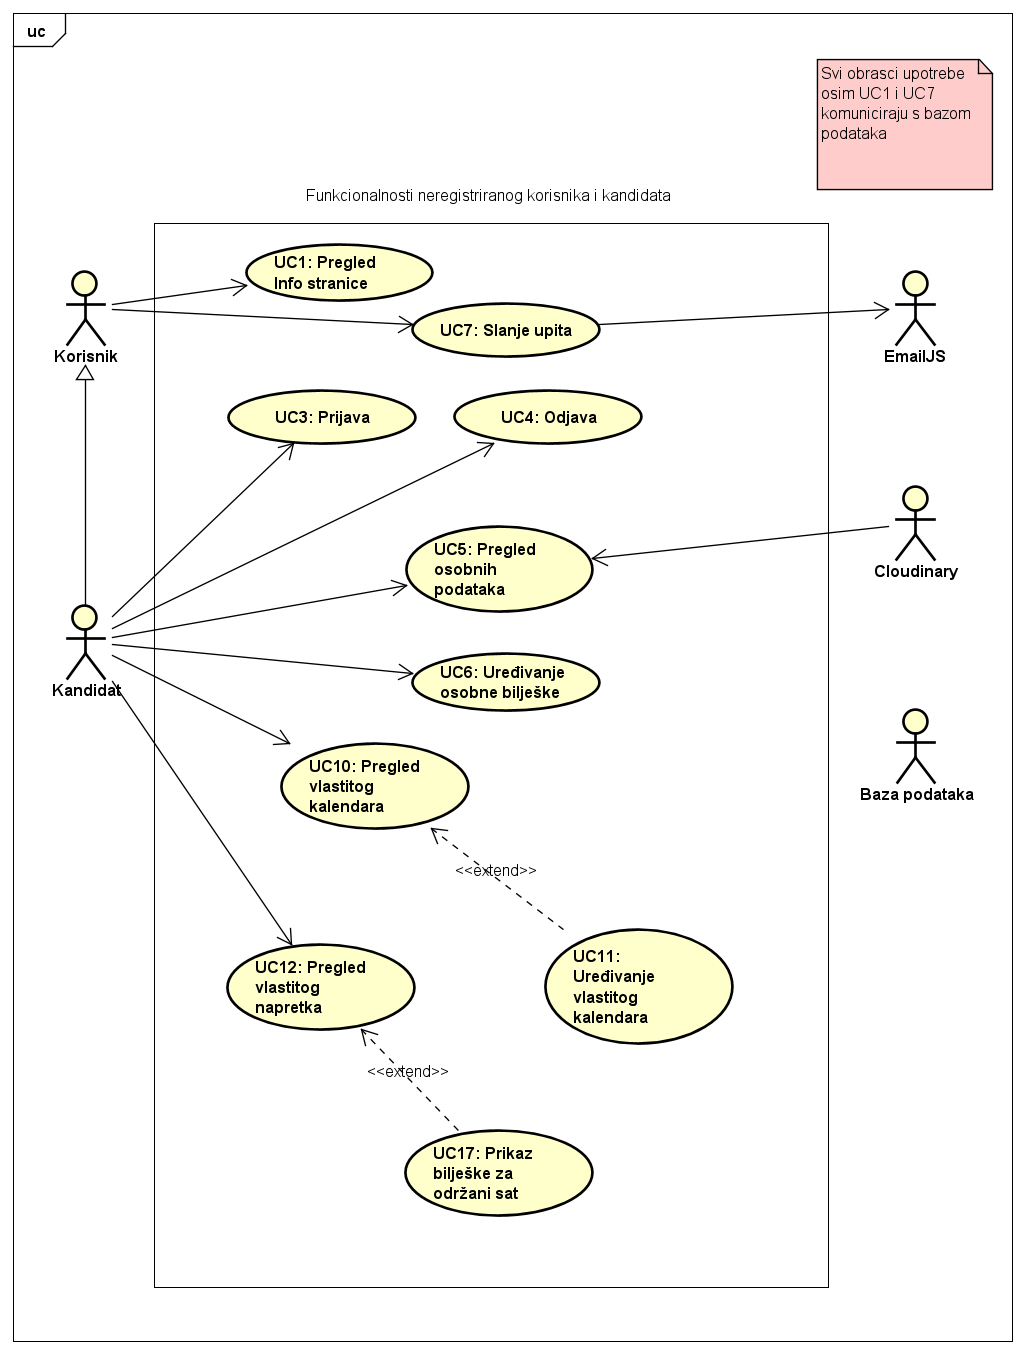
\includegraphics[width=\textwidth]{slike/UseCase Diagram3.png}
		\centering
		\vspace{-1cm}
		\caption{Dijagram obrazaca uporabe, funkcionalnost korisnika i Kandidata}
		\label{fig:promjene}
	\end{figure}

  \begin{figure}[H]
		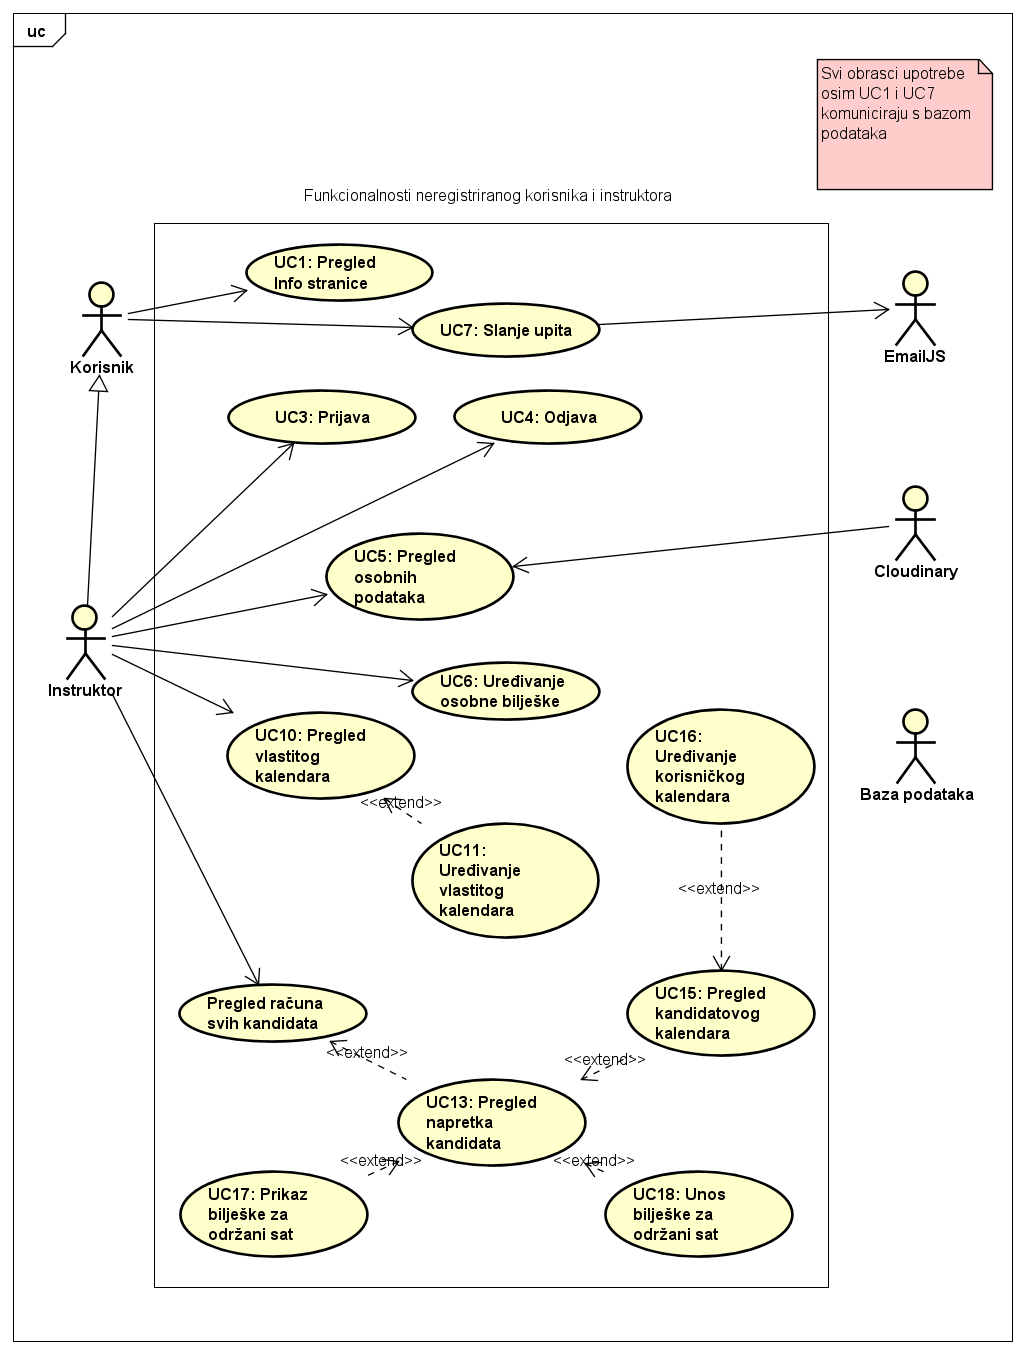
\includegraphics[width=\textwidth]{slike/UseCase Diagram2.png}
		\centering
		\vspace{-1cm}
		\caption{Dijagram obrazaca uporabe, funkcionalnost korisnika i Instruktora}
		\label{fig:promjene}
	\end{figure}

  \begin{figure}[H]
		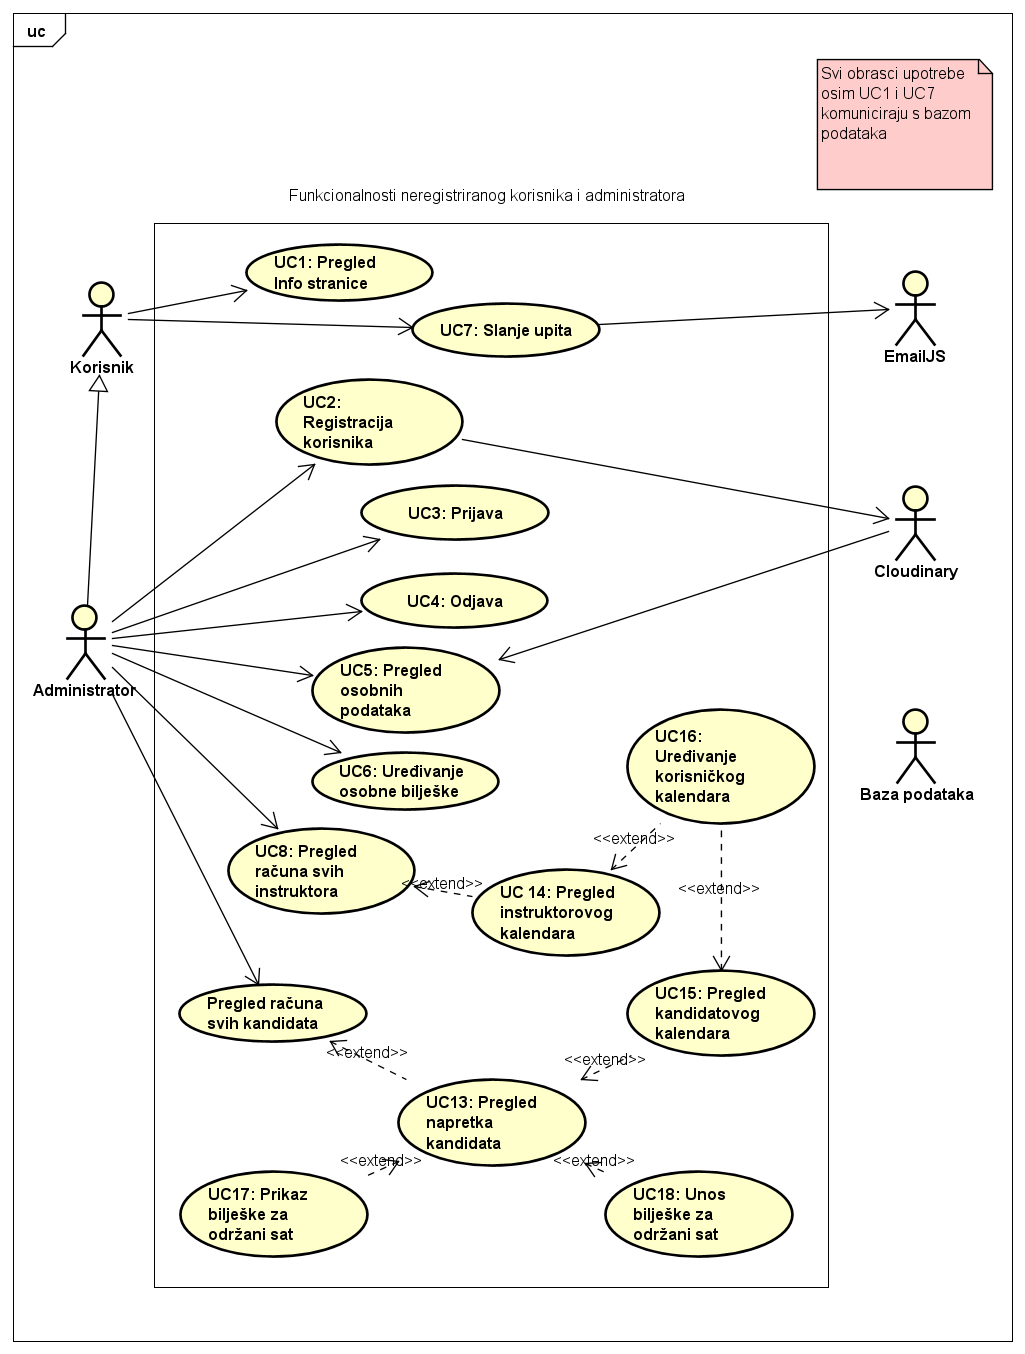
\includegraphics[width=\textwidth]{slike/UseCase Diagram1.png}
		\centering
		\vspace{-1cm}
		\caption{Dijagram obrazaca uporabe, funkcionalnost korisnika i Administratora}
		\label{fig:promjene}
	\end{figure}

 






